%%%%%%%%%%%%%%%%%%%%%%%%%%%%%%%%%%%%%%%%%%%%%%%%%%%%%%%%%%%%%%%%%%%%%%%%%%%%%%%%%%%%%%%%%%%%%%%%%%%%%%%%%%%%%%%%%%%%%%%%%%%%%%%%%%%%%%%%%%%%
%%%%%%%%%%%%%%%%%%%%%%%%%%%%%%%%%%%%%%%%%%%%%%%%%%%%%%%%%%%%%%%%%%%%%%%%%%%%%%%%%%%%%%%%%%%%%%%%%%%%%%%%%%%%%%%%%%%%%%%%%%%%%%%%%%%%%%%%%%%%
% Dies ist ein Kommentar, er wird bei der pdf-Erzeugung ignoriert.


% Dies ist eine LaTex-Vorlage für den Gebrauch im Physikalischen Praktikum I und ist als Hilfestellung zu verstehen, falls keine LaTex-Kenntnisse vorhanden sind. Einige nötige und nützliche Pakete sind bereits eingebunden und die Kapitel (\section) angelegt. Die Kapitel beinhalten teilweise Beispiele wie die Darstellung von Grafiken/Tabellen oder mathematischen Formeln sowie Referenzen/Zitationen. Nach den nun folgenden Paketeinbindungen und Definitionen können die Namen der Verfasser, der Versuchsname usw. eingegeben werden. 


%%%%%%%%%%%%%%%%%%%%%%%%%%%%%%%%%%%%%%%%%%%%%%%%%%%%%%%%%%%%%%%%%%%%%%%%%%%%%%%%%%%%%%%%%%%%%%%%%%%%%%%%%%%%%%%%%%%%%%%%%%%%%%%%%%%%%%%%%%%%
%%%%%%%%%%%%%%%%%%%%%%%%%%%%%%%%%%%%%%%%%%%%%%%%%%%%%%%%%%%%%%%%%%%%%%%%%%%%%%%%%%%%%%%%%%%%%%%%%%%%%%%%%%%%%%%%%%%%%%%%%%%%%%%%%%%%%%%%%%%%
\documentclass[a4paper,12pt,bibtotocnumbered]{scrartcl}

\usepackage[utf8]{inputenc} %Codierung des LaTeX-Dokumentes. Auf Windows-Maschinen ist statt utf8 auch ANSIC als Codierung möglich, aber unnötig, da utf8 in jeder Hinsicht besser als ANSI ist. Bei Linux: latin1 als Codierung, auf MacOS X: applemac
\usepackage[T1]{fontenc}
\usepackage[ngerman]{babel} %Deutsche Zeichen- und Umbruchsetzung
\usepackage{amsmath, amssymb,amsfonts} %AMS-TeX-Pakete. Nötig für die Definition der Mathematik-Umgebung
\usepackage{graphicx} %Nötig, um Grafiken einbinden zu können
\usepackage[bookmarks,colorlinks=true]{hyperref} %Mittels hyperref lassen sich hyperlinks innerhalb des PDF-Dokumentes benutzen. Beispiel: Mausklick im Inhaltsverzeichnis auf ein Kapitel führt zum automatischen Sprung in dieses Kapitel
\usepackage{geometry}
\usepackage{float}
%Ein Paket, mit dem sich ohne Probleme mehrseitige PDF-Dokumente ohne \includegraphics-Rumgemache einbinden lassen. Befehl: \includepdf[pages=a-b]{PDFfile.pdf}. Einzelne Seiten, oder auch alle Seiten (Option pages=-) können angewählt werden
%Wenn keine Option angegeben wird, gilt pages=1!
\usepackage[final]{pdfpages}
\usepackage{framed, color} %Framed: Paket, mittels dessen ein Rahmen um einen Bereich definiert werden kann. Color: Lässt Farbdarstellung in Schrift, Hintergrund etc. zu
\usepackage{scrlayer-scrpage} %Header für die KOMA-script -Klasse
\usepackage{siunitx} %Ein schönes Paket, um Einheiten und physikalische Größen richtig zu setzen. Z.B.  \SI{2}{\kilo\gram\per\meter\squared}
\usepackage[square,numbers]{natbib}
\usepackage{subfigure} %Mehrere Bilder in einer Figure-Umgebung

%siunitx-Konfiguration. Damit werden die richtigen Font-Einstellungen erkannt (also beispielsweise fett, kursiv etc.) und damit  ebenfalls die deutsche Zeichensetzung, insbesondere Trennungszeichen, benutzt werden. 
%Ebenso wird bei SIrange das "`to"' in "`bis"' umgewandelt, bei SIlist das "`and"' in "`und"'
\sisetup{detect-weight=true, detect-family=true,locale=DE,range-phrase={\,bis\,},list-final-separator ={\,\linebreak[0] \text{und}\,},separate-uncertainty=true,per-mode = symbol-or-fraction}
%\SI[per-mode = fraction]{1}{\meter\per\second} erzwingt auch im Fließtext die Bruchdarstellung.
\DeclareSIUnit\curie{Ci}%Zusätzliche Einheit definieren

%Hyperlinks-Setup
\hypersetup{
	colorlinks,
	linktocpage,
	citecolor=black,
	filecolor=black,
	linkcolor=black,
	urlcolor=black
}

\numberwithin{equation}{section} % Die Nummerierung von Gleichungen bekommt die jeweilige Section-Nummer als Präfix

\setlength{\parindent}{0 mm} %Einrücktiefe von neuen Absätzen
\setlength{\parskip}{2 mm} %Abstand von Absätzen



\pagestyle{scrheadings}%Kopf und Fußzeilen
\ohead{\textbf{\GRUPPENNR\ - \VERSUCHSNR}} %Header oben links auf linker Seite (ungerade Seitenzahl) und oben rechts auf rechter Seite (gerade Seitenzahl), beinhaltet gruppennummer und Versuchskürzel. Im Fall eine einseitigen Dokuments: Header oben rechts
\ihead{\VerfasserEINS\;\&\;\VerfasserZWEI} %Header oben rechts auf linker Seite und oben links auf rechter Seite. Beinhaltet die Namen der Verfasser. Im Fall eine einseitigen Dokuments: Header oben links!
\ofoot{\thepage} %Footer unten links auf linker und unten rechts auf rechter Seite, enthält die jeweilige Seitenzahl. Im Fall eines einseitigen Elements: Footer unten rechts!
\cfoot{\empty} %Mittig unten im Footer soll nichts eingetragen werden 
\ifoot{\empty} %Footer unten rechts auf linker und unten links auf rechter Seite. Hier ebenfalls leer.

%CUSTOM
\newcommand{\diff}[3][]{\frac{\mathrm{d}^{#1} {#2} }{\mathrm{d} {#3}^{#1}}}
%diff[n]{f}{t}
\newcommand{\diffp}[3][]{\frac{\partial^{#1} {#2} }{\partial {#3}^{#1}}}
%diffp[n]{f}{y}
\newcommand{\dd}{\mathrm{d}}
\usepackage[version=3]{mhchem} % Package for chemical equation typesetting


%%%%%%%%%%%%%%%%%%%%%%%%%%%%%%%%%%%%%%%%%%%%%%%%%%%%%%%%%%%%%%%%%%%%%%%%%%%%%%%%%%%%%%%%%%%%%%%%%%%%%%%%%%%%%%%%%%%%%%%%%%%%%%%%%%%%%%%%%%%%

% Hier können die individuellen Anpassungen vorgenommen werden, die sich auf das Titelblatt und die Kopfzeilen auswirken.

\newcommand{\VERSUCHSDATUM}{27.10.2020}
\newcommand{\PROTOKOLLDATUM}{\today}

\newcommand{\VerfasserEINS}{Robert Schuh}
\newcommand{\MatNoEINS}{Matrikelnummer 3452419}
\newcommand{\StudiengangEINS}{B.Sc. Physik}

\newcommand{\VerfasserZWEI}{Michelle Pfahl}
\newcommand{\MatNoZWEI}{Matrikelnummer 3465037}
\newcommand{\StudiengangZWEI}{B.Sc. Physik}

\newcommand{\BETREUER}{Luana Rubino}
\newcommand{\GRUPPENNR}{A-025}

\newcommand{\VERSUCHSNR}{E50b}
\newcommand{\VERSUCHSNAME}{Brennstoffzelle}

%%%%%%%%%%%%%%%%%%%%%%%%%%%%%%%%%%%%%%%%%%%%%%%%%%%%%%%%%%%%%%%%%%%%%%%%%%%%%%%%%%%%%%%%%%%%%%%%%%%%%%%%%%%%%%%%%%%%%%%%%%%%%%%%%%%%%%%%%%%%
% Hier beginnt die Titelseite

\begin{document}
\thispagestyle{empty}


\begin{titlepage}

\begin{center}
\Huge{\textbf{\VERSUCHSNR\ - \VERSUCHSNAME}}\\% \Huge \huge \Large \normalsize \Small usw. bestimmt die Schriftgröße.
\vspace{10mm}% Abstand
\Large{Protokoll zum Versuch des Physikalischen Praktikums I von \\ \textbf{\VerfasserEINS\;\& \VerfasserZWEI}}\\
\vspace{10mm} 
\Large{Universität Stuttgart}\\
\end{center}
\vspace{1cm}
\begin{center}
\begin{tabular}{ll}
\large{Verfasser:}		& \large{\VerfasserEINS\;(\StudiengangEINS),} \\ 
 						& \large{\MatNoEINS} \\
 						\vspace{0cm}\\
						& \large{\VerfasserZWEI\;(\StudiengangZWEI),} \\
						& \large{\MatNoZWEI} \\
						\vspace{0cm}\\
\large{Gruppennummer:}	& \large{\GRUPPENNR} \\
\vspace{0cm}\\
\large{Versuchsdatum:}	& \large{\VERSUCHSDATUM} \\
\vspace{0cm}\\
\large{Betreuer:}		& \large{\BETREUER}
\end{tabular}
\end{center}
\vspace{15mm}

\begin{center}
Stuttgart, den \PROTOKOLLDATUM
\end{center}

\end{titlepage}


\thispagestyle{empty}
%%%%%%%%%%%%%%%%%%%%%%%%%%%%%%%%%%%%%%%%%%%%%%%%%%%%%%%%%%%%%%%%%%%%%%%%%%%%%%%%%%%%%%%%%%%%%%%%%%%%%%%%%%%%%%%%%%%%%%%%%%%%%%%%%%%%%%%%%%%%%%%%
%Mittels des untenstehenden einfachen Befehls wird ein Inhaltsverzeichnis angelegt. LaTeX erstellt das Inhaltsverzeichnis völlig automatisch anhand der Überschriften für Kapitel, Unterkapitel etc. Das Dokument muss
%unter Umständen zweimal neu gesetzt werden, damit Änderungen in den Überschriften auch im Inhaltsverzeichnis auftauchen!
%%%%%%%%%%%%%%%%%%%%%%%%%%%%%%%%%%%%%%%%%%%%%%%%%%%%%%%%%%%%%%%%%%%%%%%%%%%%%%%%%%%%%%%%%%%%%%%%%%%%%%%%%%%%%%%%%%%%%%%%%%%%%%%%%%%%%%%%%%%%%%%%
\tableofcontents 
%%%%%%%%%%%%%%%%%%%%%%%%%%%%%%%%%%%%%%%%%%%%%%%%%%%%%%%%%%%%%%%%%%%%%%%%%%%%%%%%%%%%%%%%%%%%%%%%%%%%%%%%%%%%%%%%%%%%%%%%%%%%%%%%%%%%%%%%%%%%%%%%
\clearpage %Neue Seite, davor werden alle noch ausstehenden Grafiken/Tabellen platziert.

\renewcommand{\thepage}{\arabic{page}}
\setcounter{page}{1}


%%%%%%%%%%%%%%%%%%%%%%%%%%%%%%%%%%%%%%%%%%%%%%%%%%%%%%%%%%%%%%%%%%%%%%%%%%%%%%%%%%%%%%%%%%%%%%%%%%%%%%%%%%%%%%%%%%%%%%%%%%%%%%%%%%%%%%%%%%%%
%%%%%%%%%%%%%%%%%%%%%%%%%%%%%%%%%%%%%%%%%%%%%%%%%%%%%%%%%%%%%%%%%%%%%%%%%%%%%%%%%%%%%%%%%%%%%%%%%%%%%%%%%%%%%%%%%%%%%%%%%%%%%%%%%%%%%%%%%%%%
%%%%%%%%%%%%%%%%%%%%%%%%%%%%%%%%%%%%%%%%%%%%%%%%%%%%%%%%%%%%%%%%%%%%%%%%%%%%%%%%%%%%%%%%%%%%%%%%%%%%%%%%%%%%%%%%%%%%%%%%%%%%%%%%%%%%%%%%%%%%

% Die erste eckige Klammer ist optional, die darin angegebene Bezeichnung steht im Inhaltsverzeichnis anstelle des hinteren (längeren) Namens.
\section[Versuchsziel]{Versuchsziel und Versuchsmethode}
In diesem Versuch werden die Effizienz und Leistung einer Brennstoffzelle und eines Elektrolyseurs sowie die Leckrate des Gesamtsystems gemessen.
\section{Grundlagen}
Eine Brennstoffzelle ist ein Apparat, der eine Reaktion von zwei Stoffen elektrochemisch kontrolliert ablaufen lässt und die Reaktionsenergie als elektrische Energie freigibt. Es gibt Brennstoffzellen für verschiedene exotherme Reaktionen, die Brennstoffzelle in diesem Versuch arbeitet mit Wasserstoff und Sauerstoff:
\begin{equation}\label{wasser}
\ce{H_2(g) + \frac{1}{2}O_2(g) -> H_2O(l)}
\end{equation}
Ein Elektrolyseur verwendet elektrische Energie, um eine endotherme Elektrolysereaktion durchzuführen. Der Elektrolyseur in diesem Versuch spaltet Wasser und kehrt Reaktion (\ref{wasser}) um.\\
Um die Reaktion kontrolliert ablaufen zu lassen, wird sie in zwei Teilreaktionen getrennt:
\begin{align}
\ce{H_2 &-> 2H^+ + 2e^-} \\
\ce{\frac{1}{2}O_2 + 2H^+ + 2e^- &->H_2O}
\end{align}
Diese Teilreaktionen laufen in der Brennstoffzelle räumlich getrennt auf zwei verschiedenen Seiten einer für $\ce{H^+}$-Ionen durchlässigen Membran ab. Die Elektronen müssen über elektrische Leitungen fließen, was nur möglich ist wenn ein an die Zelle angeschlossener elektrischer Verbraucher Strom fließen lässt. Kann nicht genug Strom fließen, so baut sich an den Elektroden eine Spannung auf. Damit wird die Reaktion geregelt und die Reaktionsenergie wird elektrisch an den Verbraucher abgegeben.\\
In einem Elektrolyseur wird umgekehrt eine Spannung an zwei Elektroden in $\ce{H_2O}$ angelegt. Dadurch läuft Reaktionen der Brennstoffzelle umgekehrt ab. \\
Es kann eine Protonendurchlässige Membran wie in der Brennstoffzelle verwendet werden, oder man kann die Elektroden in zwei Seiten eines mit saurem bzw. alkalischem Wasser gefüllten U-Rohrs installieren und das ionenreiche Wasser selbst als "Membran" nutzen, die keine Gase $\ce{H_2},\ce{O_2}$ hindurchlässt aber Protonen in Form von $\ce{H_3O^+}$ bzw. $\ce{OH^-}$ transportieren kann.\\



\section[Messprinzip]{Messprinzip und Versuchsablauf}

\subsection{Aufbau und Geräteliste}

\subsection{Versuchsablauf}

\section[Messwerte]{Messwerte}
\section[Auswertung]{Auswertung}
\section[Fehlerrechnung]{Fehlerrechnung}
\section[Zusammenfassung]{Zusammenfassung}
\begin{thebibliography}{999}
\bibitem{Anleitung} Versuchsanleitung zum Physik-Praktikum (Abgerufen am 26.10.2020) 
\end{thebibliography}

% Für Dokumente mit mehr Referenzen empfiehlt es sich, auf eine separate .bib -Datei umzusteigen, die alle Referenzen enthält. Diese Referenzen können bei den meisten wissenschaftlichen Publikationen direkt über "BibTex-Export" oder ähnliches heruntergeladen werden. Anstelle von \begin{thebibliography}...\bibitem{}..\bibitem{}..\end{thebibliography} muss dann lediglich \bibliography{Dateiname.bib} eingebunden werden.

\section{Anhang}
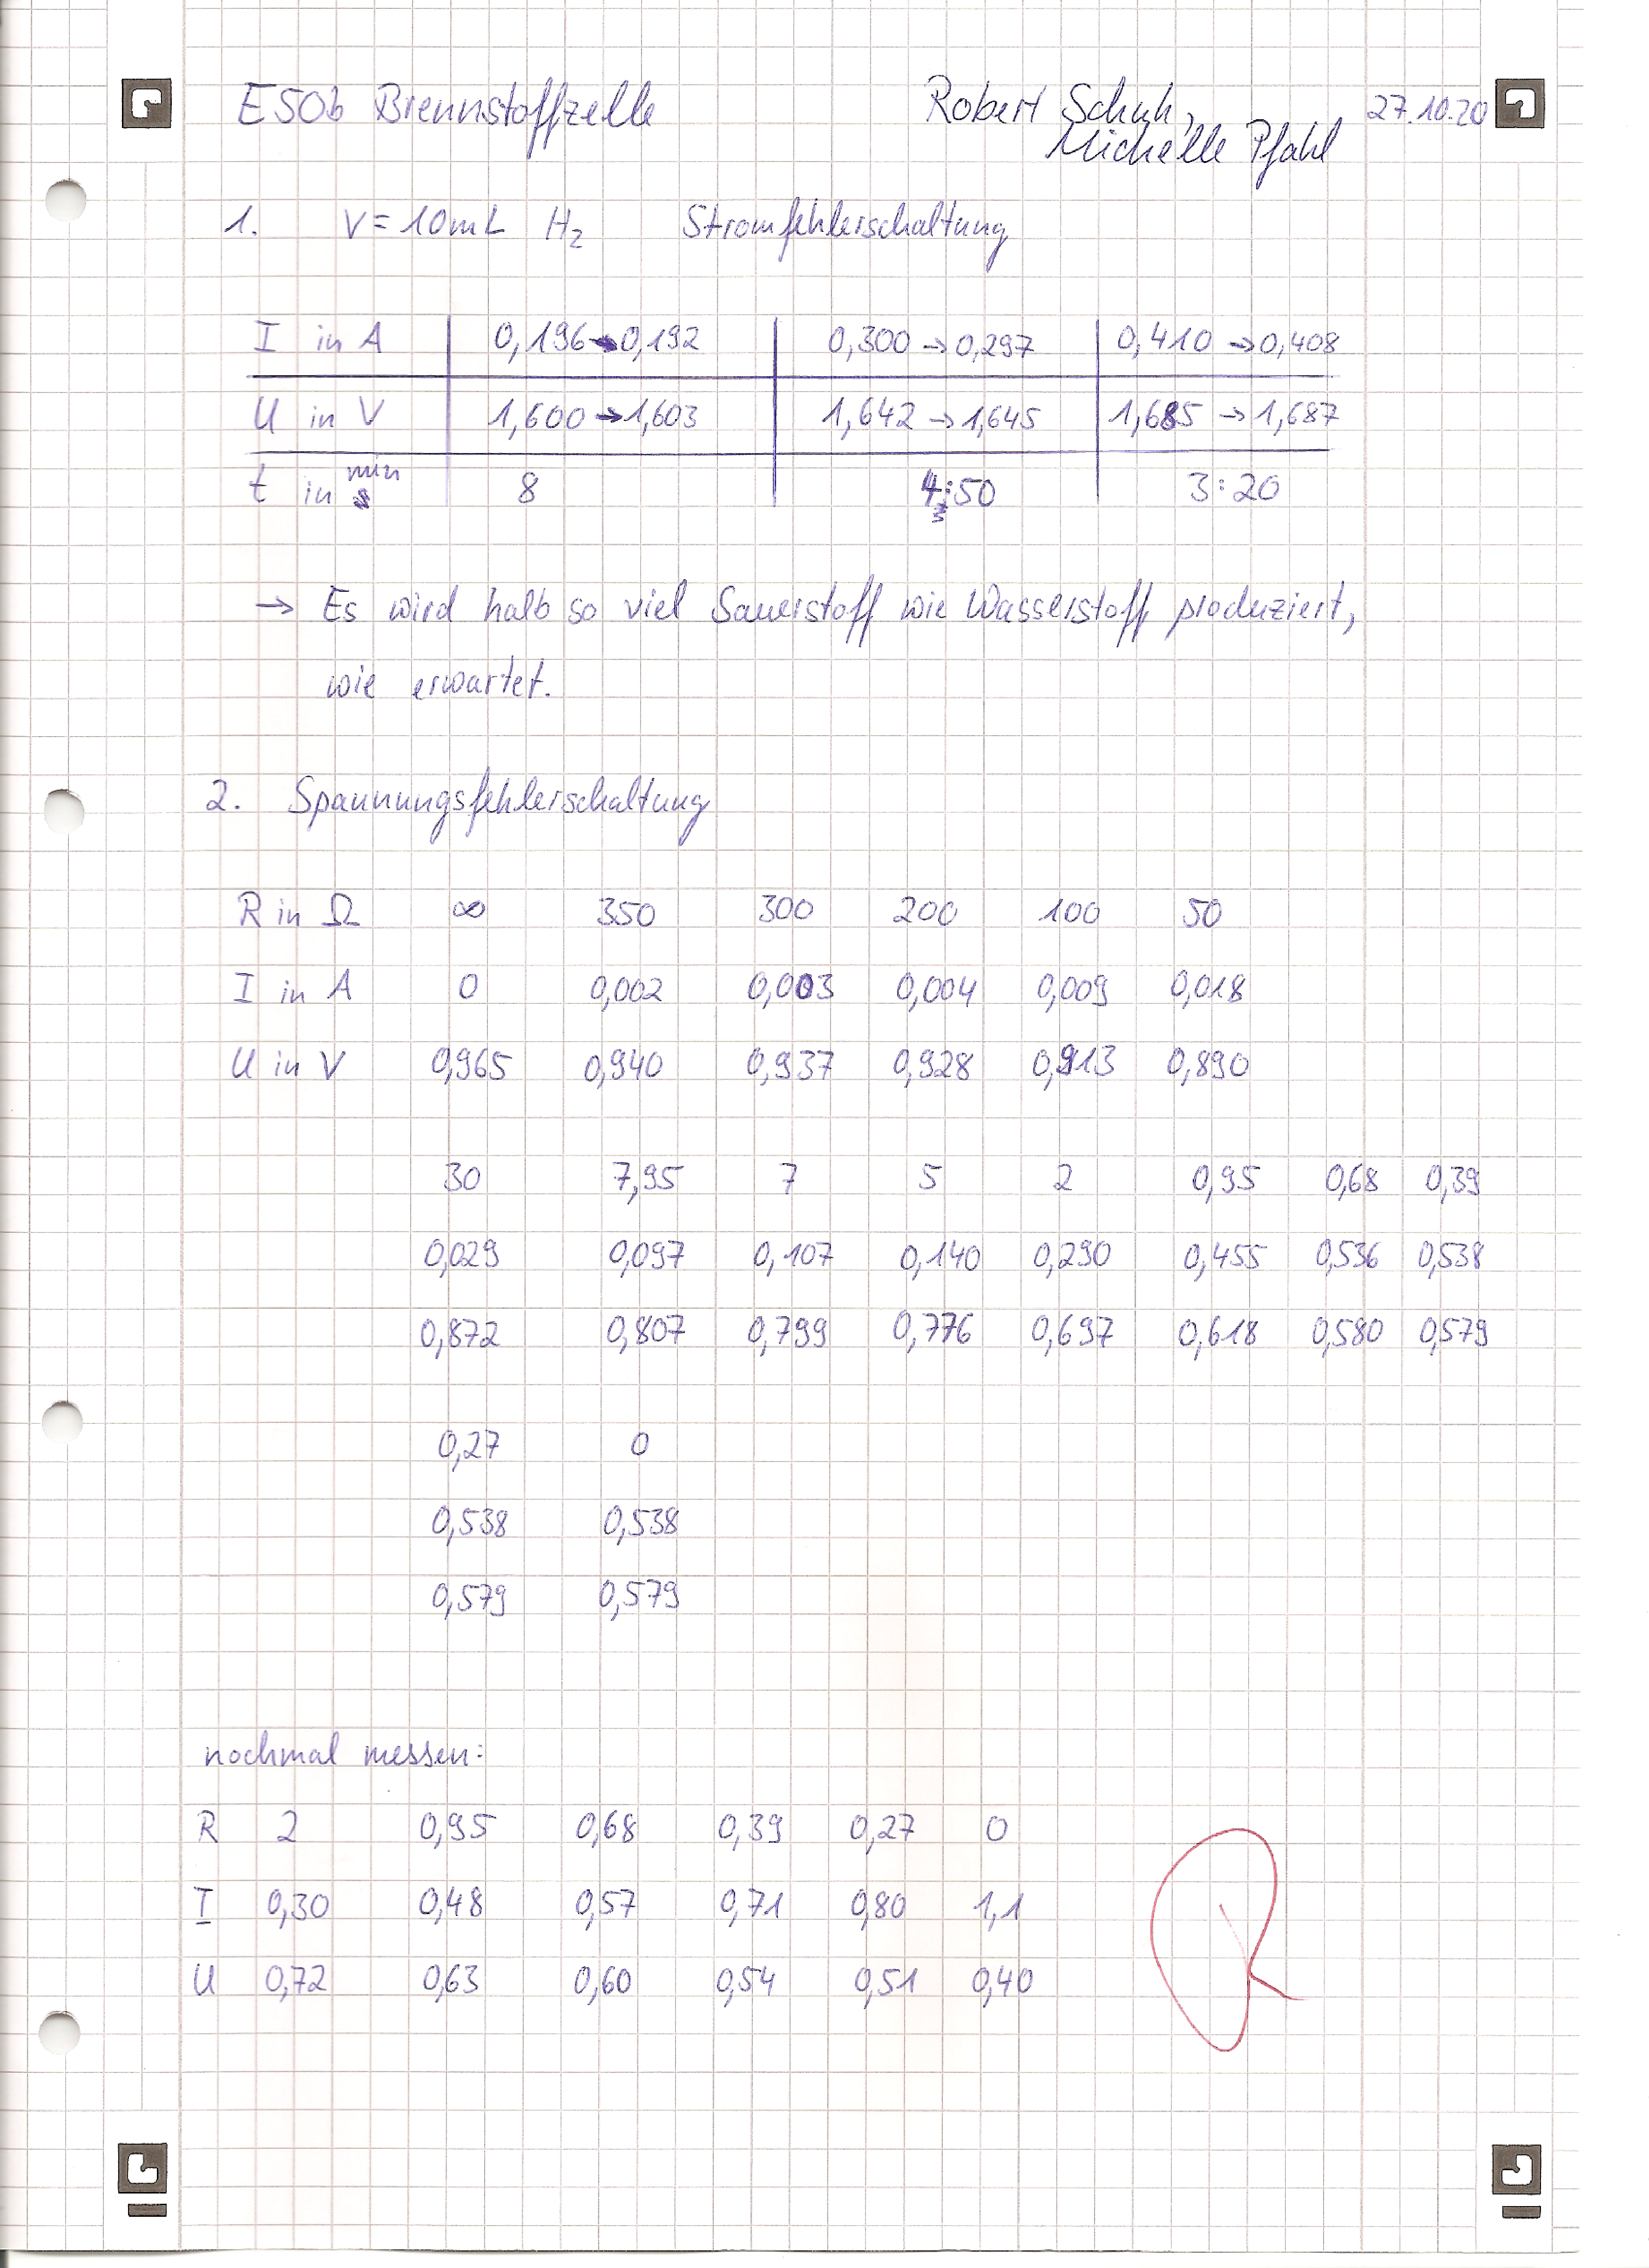
\includepdf[pages=-]{E50b Messdaten.pdf}


\end{document}
